\documentclass{beamer}

\usepackage{../defs}

\usepackage{mathrsfs}

\usepackage{xcolor}

\newcommand{\blue}[1]{\textcolor{blue}{#1}}
\newcommand{\red}[1]{\textcolor{red}{#1}}
\newcommand{\green}[1]{\textcolor{green}{#1}}

\usetheme{Montpellier}
\usecolortheme{spruce}

\title{Application of Convex Relaxation on Low-rank Optimization Problems}
\author{GKxx, Jayncp, ZYP}
\date{\today}

\AtBeginSubsection{
    \begin{frame}{Contents}
        \tableofcontents[currentsection, currentsubsection]
    \end{frame}
}

\begin{document}

\begin{frame}
    \maketitle
\end{frame}

\begin{frame}{Contents}
    \tableofcontents
\end{frame}

\section{Convex Relaxation}

\subsection{Introduction}

\begin{frame}{Solve Non-convex Problems}
    Typical ways of solving non-convex problems:
    \begin{itemize}
        \item Descent methods
        \begin{itemize}
            \item Block coordinate descent method
            \item Gradient descent method
            \item Steepest descent method
            \item \dots
        \end{itemize}
        \item Successive convex approximation method
        \item \blue{Convex relaxation method}
    \end{itemize}
\end{frame}

\section{Low-rank Optimization}

\subsection{Examples}

\begin{frame}{Non-rigid Structure-from-Motion}
    \[\begin{aligned}
        \minimize & \rank\left(S^\sharp\right)\\
        \subjectto & W=RS,
    \end{aligned}\]
    where \(S^\sharp:=\bvec{P_X & P_Y & P_Z}\left(I_3\otimes S\right)\).
\end{frame}

\begin{frame}{Latent Low-rank Representation Model}
    \[\begin{aligned}
        \minimize & \rank Z+\rank L\\
        \subjectto & X=XZ+LX.
    \end{aligned}\]
    \pause
    The corresponding nuclear norm minimization formulation:
    \[\begin{aligned}
        \minimize & \norm Z_\ast+\norm L_\ast\\
        \subjectto & X=XZ+LX.
    \end{aligned}\]
\end{frame}

\subsection{Equality Constraints}

\begin{frame}{Problem Formulation}
    \begin{definition}[Low-rank minimization]
        Let \(\mathcal A:\R^{m\by n}\to\R^p\) be a linear map and \(b\in\R^p\). The low-rank minimization problem is of the form
        \[\begin{aligned}
            \minimize & \rank X\\
            \subjectto & \mathcal A(X)=b.
        \end{aligned}\]
    \end{definition}
    \pause
    \begin{itemize}
        \item \(\rank(\cdot)\) is non-convex.
        \item Write \(\mathcal A(\cdot)\) as multiplication by a matrix \(A\), and \(\mathcal A(X)\) is equivalent to \(A\operatorname{vec}(X)\).
    \end{itemize}
\end{frame}

\begin{frame}{Notations}
    \begin{definition}[Support]
        The \emph{support} of a vector \(x\) is defined as \(\supp(x)=\left\{i\mid x_i\neq 0\right\}\).
    \end{definition}
    \begin{definition}[Nuclear norm]
        Given \(X\in\R^{m\by n}\) and \(q=\min\{m,n\}\), the \emph{nuclear norm} of \(X\) is defined as
        \[\norm{X}_\ast=\sum_{i=1}^k\sigma_i(X),\]
        where \(\sigma_i(X)\) is the \(i\)-th singular value of \(X\).
    \end{definition}
\end{frame}

\begin{frame}{Notations}
    \begin{definition}[Approximately sparse vectors]
        The set of approximately sparse vectors with support \(S\) is
        \[C(S):=\left\{\Delta\in\R^d\mid\norm{\Delta_{\bar S}}_1\leqslant\norm{\Delta_S}_1\right\},\]
        where \(S\subseteq [d]:=\left\{1,2,\cdots,d\right\},\bar S=[d]-S\) and \(\Delta_S\) is \(\Delta\) restricted to \(S\), i.e.
        \[\left(\Delta_S\right)_i=\begin{cases}
            \Delta_i,&i\in S\\
            0,&\otherwise.
        \end{cases}\]
    \end{definition}
\end{frame}

\begin{frame}{Relaxation by Nuclear Norm}
    \[\begin{aligned}
        \minimize & \norm X_\ast:=\sum_{i=1}^k\sigma_i(X)\\
        \subjectto & \mathcal A(X)=b.
    \end{aligned}\]
    \begin{itemize}
        \item A convex relaxation
        \item Under what circumstances is this relaxation tight?
    \end{itemize}
\end{frame}

\begin{frame}{Relaxation by Nuclear Norm}
    \begin{theorem}
        Suppose \(X_0\) is the optimal point of a low rank representation problem with \(\rank X_0=r\) and SVD \(X_0=U\Sigma V^T\), \(k=\min\{m,n\}\), \(S=[r]\), \(\bar S=[k]-S\) and \(\mathcal B:\R_{\geqslant 0}^k\to\R^p\),
        \[\mathcal B:\left(x_1,\cdots,x_k\right)\mapsto\mathcal A\left(U\begin{pmatrix}
            \diag(x_1,\cdots,x_k) & 0\\
            0 & 0
        \end{pmatrix}_{m\by n}V^T\right).\]
        If \(\Null{\mathcal B}\cap C(S)=\{0\}\), then the optimal point of the relaxation given by nuclear norm is the same as that of the original problem.
    \end{theorem}
    \begin{itemize}
        \item \(\Null{\mathcal B}\cap C(S)=\{0\}\): Restricted Nullspace Property (RNP).
    \end{itemize}
\end{frame}

\subsection{Positive Semidefinite Constraints}

\begin{frame}{Positive Semidefinite Requirement}
    Further require the variable \(X\) to be positive semidefinite:
    \[\begin{aligned}
        \minimize & \Tr X\\
        \subjectto & \mathcal A(X)=b\\
        & X\succeq 0.
    \end{aligned}\]
    \begin{itemize}
        \item An SDP problem.
    \end{itemize}
\end{frame}

\begin{frame}{Positive Semidefinite Requirement}
    To reduce the number of constraints, we may punish the violation of the equality constraint on the objective function:
    \[\begin{aligned}
        \minimize & \alpha\Tr X+\frac12\norm{\mathcal A(X)-b}\\
        \subjectto & X\succeq 0.
    \end{aligned}\]
    \begin{itemize}
        \item \(\alpha\) is a scalar regularization variable that directly trades off goodness for complexity of fit.
        \item Its optimal value depends upon the assumed noise level in practice.
    \end{itemize}
\end{frame}

\subsection{Relaxation}

\begin{frame}{An Easier Problem}
    The \(\ell_0\)-minimization problem:
    \[\begin{aligned}
        \minimize & \norm x_0\\
        \subjectto & Ax=y,
    \end{aligned}\]
    where \(A\in\R^{n\by d}\) and \(y\in\R^n\).
    \begin{itemize}
        \item The \(\ell_0\)-norm \textbf{isn't} a real norm.
        \item \(\norm x_0\) is \textbf{not} convex.
        \item \(\ell_0\)-minimization problem is NP-hard.
    \end{itemize}
\end{frame}

\begin{frame}{Exact 3-cover Problem}
    \begin{definition}[Exact 3-cover]
        Given a collection \(\left\{T_i\right\}\) of \(3\)-element subsets \(\{1,\cdots,n\}\), the \emph{exact 3-cover problem} is to find an exact cover of \(\left\{1,\cdots,n\right\}\) and a set \(Z\subseteq\{1,\cdots,d\}\) such that
        \[\bigcup_{j\in Z}T_j=\{1,2,\cdots,n\}\]
        and \(T_i\cap T_j=\varnothing\) for \(i\neq j\in Z\).
    \end{definition}
    \begin{itemize}
        \item NP-hard.
        \item Could be reduced to \(\ell_0\)-minimization, thus the latter is NP-hard.
    \end{itemize}
\end{frame}

\begin{frame}{Relaxation}
    Relax to the \(\ell_1\)-minimization problem:
    \[\begin{aligned}
        \minimize & \norm x_1\\
        \subjectto & Ax=y.
    \end{aligned}\]
    \begin{itemize}
        \item A convex relaxation.
        \item Under what circumstances is this relaxation tight?
    \end{itemize}
\end{frame}

\begin{frame}{Relaxation}
    \begin{theorem}
        Let \(x^\ast\) be the optimal solution of the \(\ell_0\)-minimization problem and \(\supp(x)=S\). If \(A\) satisfy the restricted nullspace property with respect to \(S\), then the optimal solution to the associated \(\ell_1\)-minimization problem is also \(x^\ast\).
    \end{theorem}
    \begin{proof}[Proof Sketch]
        Let \(\Delta=\widehat x-x^\ast\) be the error vector, where \(\widehat x\) is the solution to the \(\ell_1\)-minimization problem. Then \(\Delta\in\Null A\). We only need to show \(\Delta\in C(S)\).
    \end{proof}
\end{frame}

\begin{frame}{Restricted Isometry Property}
    \begin{definition}[Restricted Isometry Property, RIP]
        A matrix \(A\) satisfies the \((s,\delta)\)-RIP if for all \(s\)-sparse vectors \(x\) (i.e. \(\norm x_0\leqslant s\)), we have
        \[(1-\delta)\norm x_2^2\leqslant\norm{Ax}_2^2\leqslant(1+\delta)\norm x_2^2.\]
    \end{definition}
    \begin{itemize}
        \item \(A\) acts like an isometry on sparse vectors.
    \end{itemize}
\end{frame}

\begin{frame}{RIP \(\Rightarrow\) RNP}
    \begin{theorem}
        If the matrix \(A\) has the \((s,\delta)\)-RIP, then it also has the restricted nullspace property for all subsets \(S\) of cardinality \(\abs S\leqslant s\).
    \end{theorem}
\end{frame}

\begin{frame}{Relationship}
    \begin{center}
        \begin{tabular}{|ll|}
            \hline
            \(\norm x_0\): & Number of nonzero elements in \(x\).\\
            \(\rank(X)\): & Number of nonzero singular values of \(X\).\\
            \hline\hline
            \(\norm x_1\): & Sum of absolute values of components of \(x\).\\
            \(\norm X_\ast\): & Sum of singular values of \(X\).\\
            \hline
        \end{tabular}
    \end{center}
\end{frame}

\section{Solution}

\subsection{Projected Subgradient Methods}

\begin{frame}{Subgradient}
    The nuclear norm is not differentiable.
    \pause
    \begin{definition}[Subgradient]
        Let \(f:\R^n\to\R\) and its subgradient at \(x_0\) is a set defined by
        \[\partial f\left(x_0\right):=\left\{d\in\R^n\mid f(y)\geqslant f\left(x_0\right)+d^T\left(y-x_0\right),\forall y\in\R^n\right\}.\]
    \end{definition}
    \pause
    \begin{itemize}
        \item If \(f\) is continuous at \(x_0\), then \(\partial f\left(x_0\right)\neq\varnothing\).
    \end{itemize}
\end{frame}

\begin{frame}{Subgradient}
    \begin{center}
        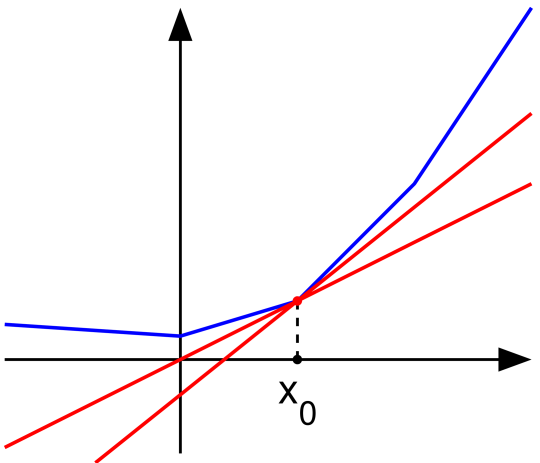
\includegraphics[width=0.7\textwidth]{img/Subderivative_illustration.png}
    \end{center}
\end{frame}

\begin{frame}{Subgradient}
    Subgradient of the nuclear norm at \(X_0\):
    \[\partial\norm{X_0}_\ast=\left\{UV^T+W\right\},\]
    where \(W\) and \(X\) have orthogonal row/column spaces, \(\norm W\leqslant 1\), and \(X_0=U\Sigma V^T\) is the SVD of \(X_0\).
\end{frame}

\end{document}